\section{Visualización de datos}\label{sec:impl_visualizacion}
Una vez se cuentan con datos en Elasticsearch, se puede comenzar el desarrollo
de la visualización de los mismos mediante Kibana. Para ello, se han desarrollado
paneles de visualización que permiten la monitorización de los datos en tiempo
real y la creación de informes y \textit{dashboards} personalizados para cada
modelo de datos contemplado.

Esta sección de la memoria documenta el desarrollo de las siguientes historias
de usuario, siguiendo la planificación establecida en la sección \fullref{sec:planif_inicial}:

\begin{table}[H]
	\centering
	\begin{tabular}{|p{0.7\linewidth}|c|c|}
		\hline
		\textbf{Nombre} & \textbf{Prioridad} & \textbf{Tamaño} \\
		\hline
		\hline
		Como trabajador de Okticket, quiero poder ver y consultar datos internos de la empresa & P1\cellcolor{orange!50} & M\cellcolor{yellow!50} \\
		\hline
		Como desarrollador de Okticket, quiero poder ver el estado general de la infraestructura & P1\cellcolor{orange!50} & M\cellcolor{yellow!50} \\
		\hline
  \end{tabular}
  \caption{Lista de HUs cumplimentadas con la visualización de datos}
  \label{tab:impl_visualizacion}
\end{table}


\newpage{}
\subsection{Desarrollo de dashboards}
Para el desarrollo de los dashboards, se han seguido los siguientes pasos:

\begin{enumerate}
    \item \textbf{Identificación de métricas clave}: se identifican las
    métricas más relevantes incluyendo: número de solicitudes, latencia,
	códigos de estados, tipos de errores, etc.

    \item \textbf{Diseño de visualizaciones}: Para cada métrica identificada,
    se decide el tipo de visualización más adecuada. Por ejemplo, gráficos
	temporales para métricas que varían con el tiempo, mapas para visualizar
	distribuciones geográficas, etc.

    \item \textbf{Creación de paneles}: se crean dos paneles principales:
    \begin{itemize}
        \item \textbf{Dashboard de estado general de infraestructura}: Incluye
        visualizaciones del tráfico total, distribución de carga, y estado de
        salud del servicio dependiendo de la infraestructura.
        \item \textbf{Dashboard de métricas detalladas}: muestra información
        más específica como latencias por URL, análisis de errores, tendencias
		temporales, etc.
    \end{itemize}

    \item \textbf{Configuración de filtros y controles}: gracias al sistema de
		filtros y controles de Kibana, los usuarios pueden personalizar las
		visualizaciones para ver solo la información relevante, además de
		ajustar el rango temporal de los datos. (ver \fullref{sec:manual_usuario}).
\end{enumerate}

\subsubsection{Personalización y acceso}
Actualmente, todos los usuarios tienen acceso completo a los dashboards
desarrollados. Se ha identificado la necesidad futura de implementar un sistema
de gestión de usuarios y permisos en Kibana. Esto permitirá asegurar que cada
usuario tenga acceso solo a los dashboards y datos relevantes para su función,
especialmente importante para la visualización de métricas sensibles de los
balanceadores de carga.

La implementación de este sistema de permisos, así como la capacidad de que los
usuarios puedan personalizar sus propios dashboards, se ha planificado como una
tarea para futuras iteraciones del proyecto.


\newpage{}
\subsection{Ejemplos de dashboards}
\begin{figure}[H]
	\centering
	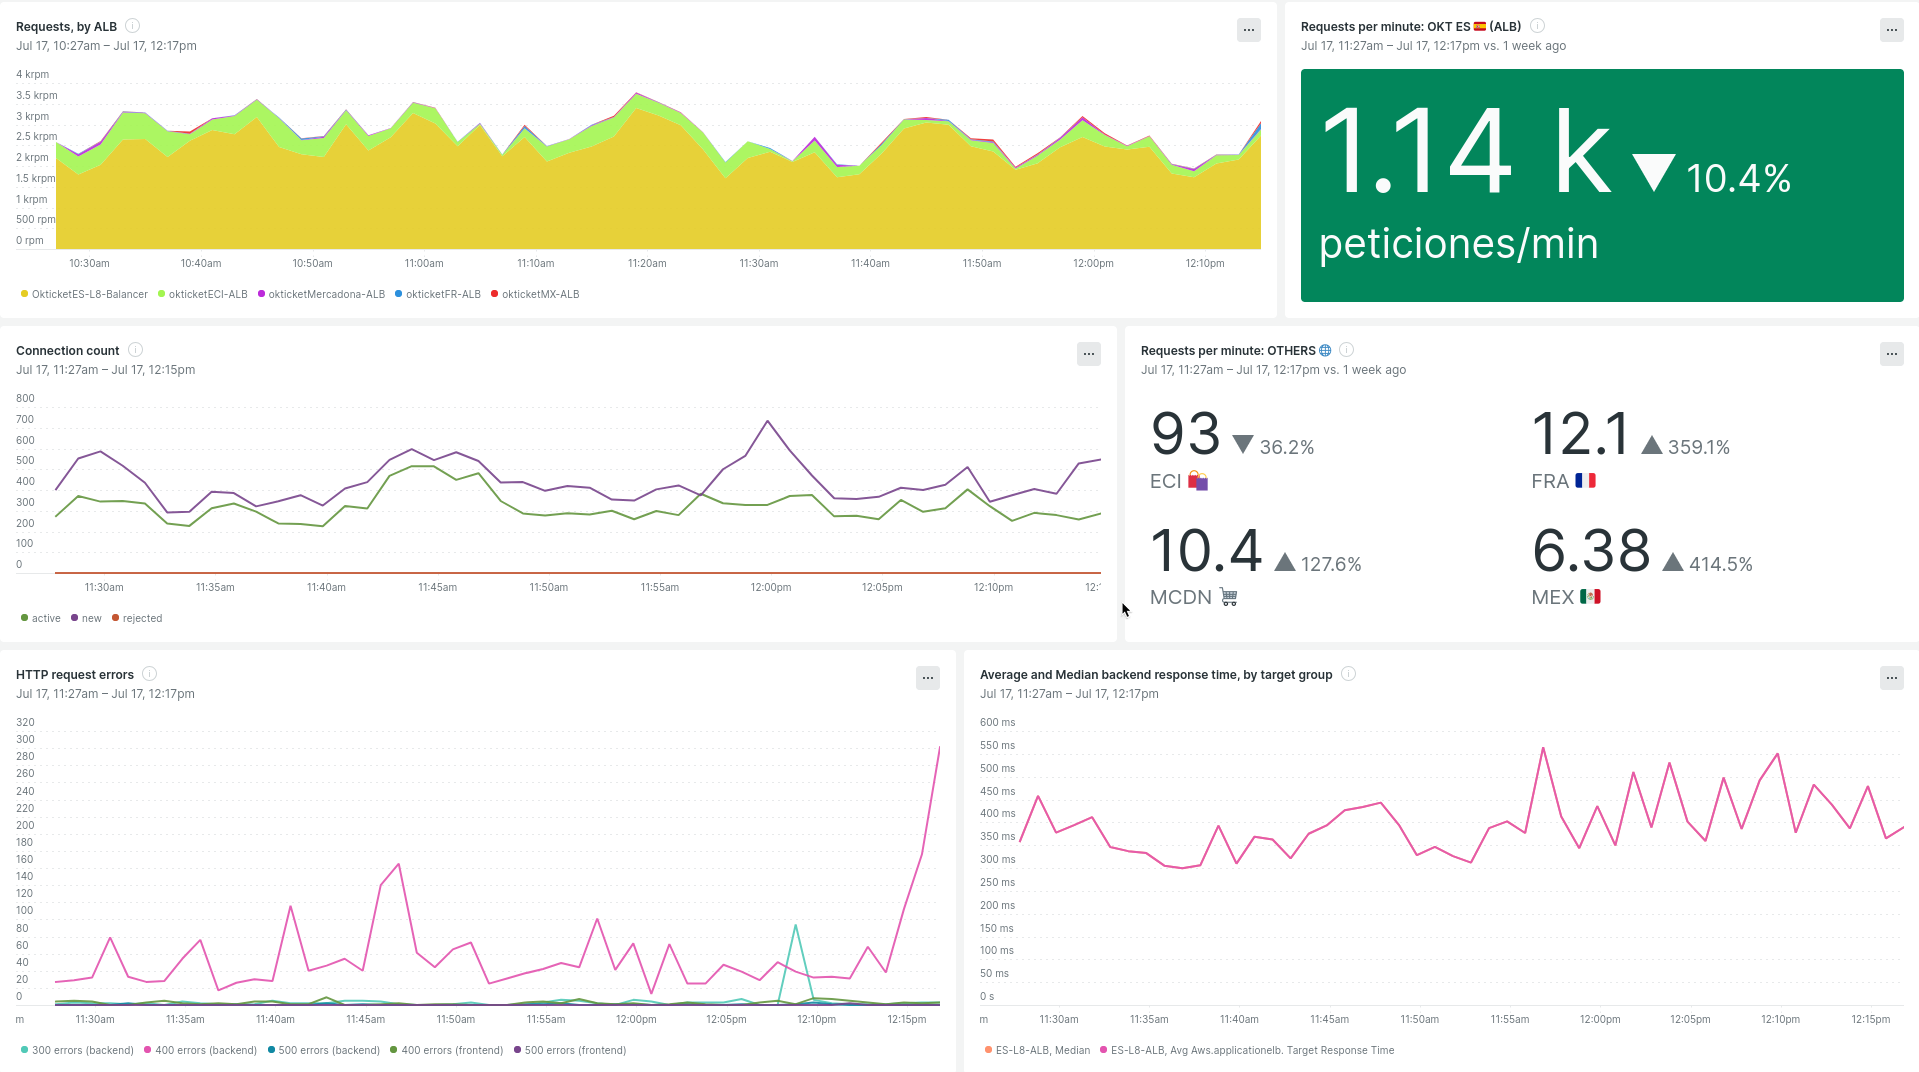
\includegraphics[width=\textwidth]{impl/dashboard_a.png}
	\caption{Dashboard de estado general de infraestructura}
	\label{fig:dashboard_a}
\end{figure}

\begin{figure}[H]
	\centering
	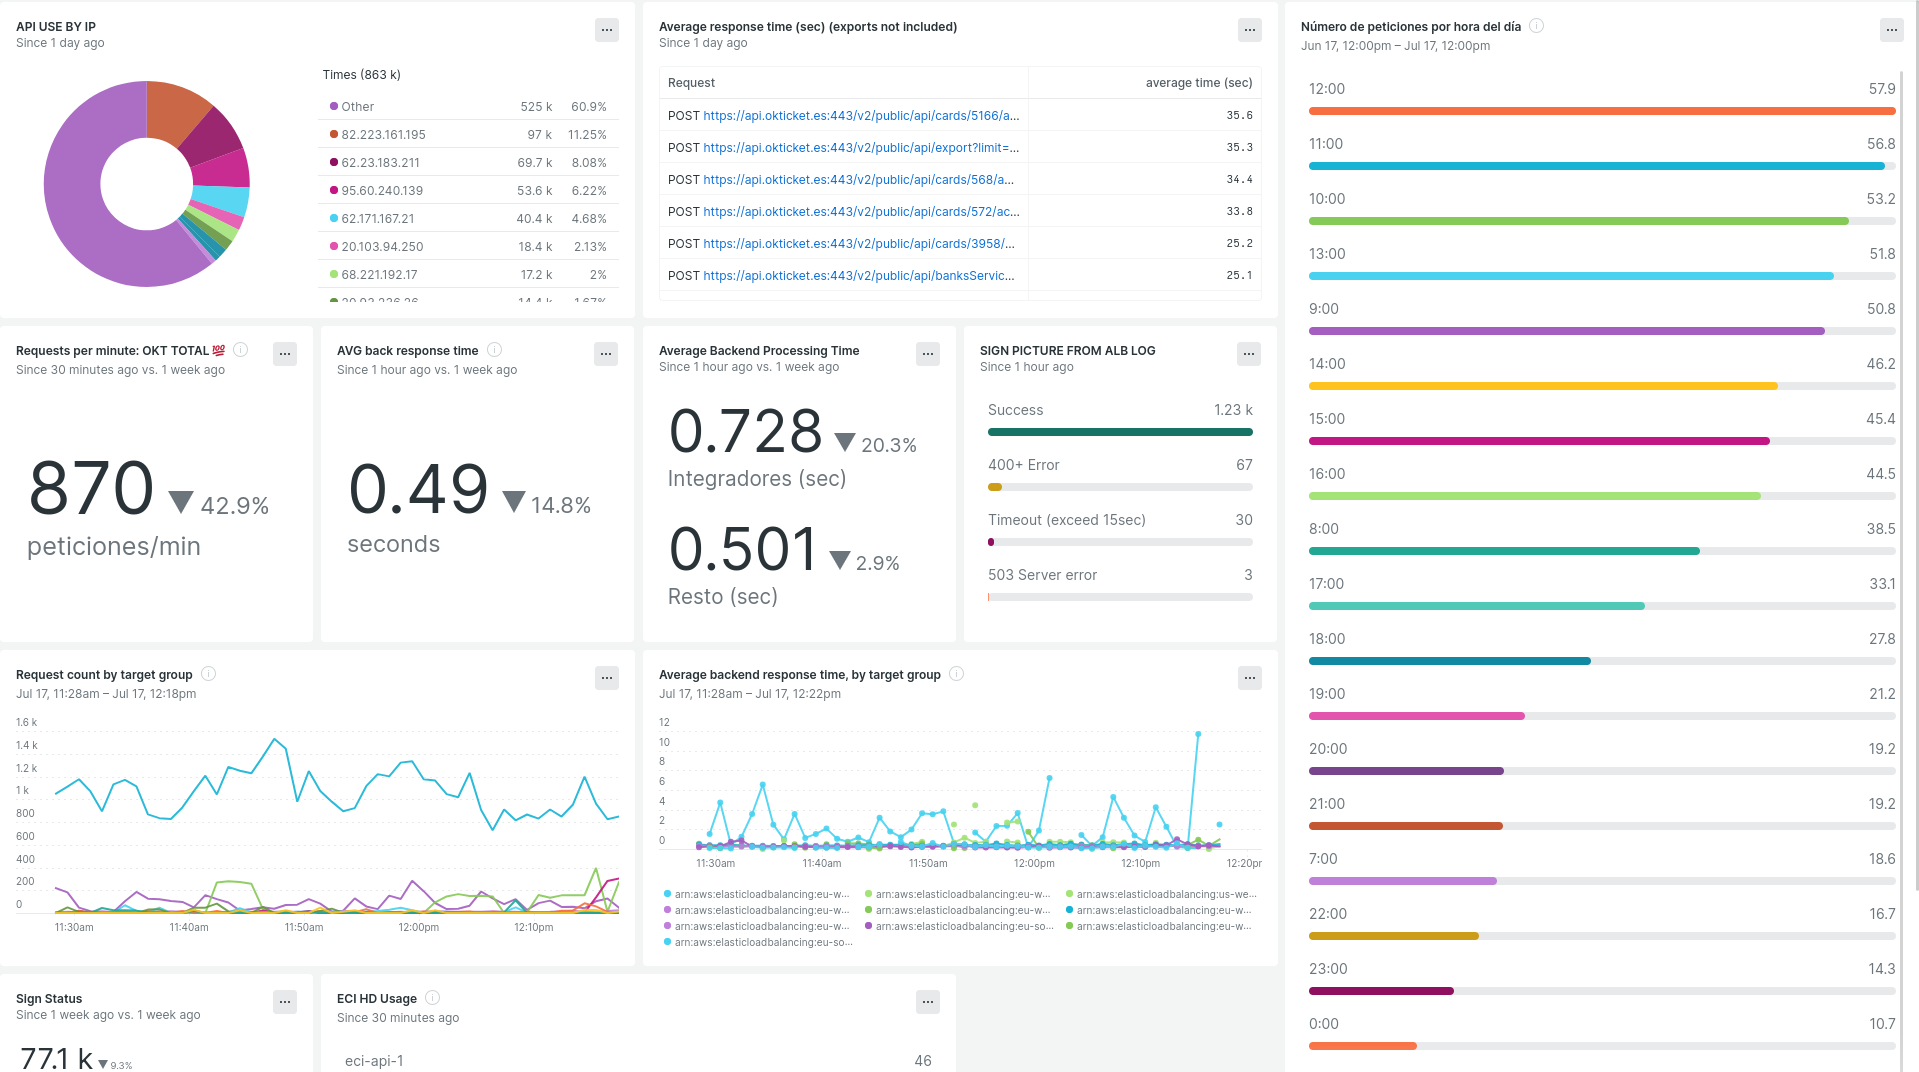
\includegraphics[width=\textwidth]{impl/dashboard_b.png}
	\caption{Dashboard de métricas detalladas}
	\label{fig:dashboard_b}
\end{figure}
